\documentclass{scrartcl}

\usepackage[utf8x]{inputenc}
\usepackage{graphicx}
\usepackage{booktabs}
\usepackage{titling}
\usepackage{xcolor}
\usepackage{amsmath}
\usepackage{amsfonts}
% 

\setlength{\droptitle}{-7.5em}

\title{Causal Inference for Policy Evaluation\\
\Large{Assignment 2}}
\author{Marco Gortan, Felix Schulz, Benjamin Weggelaar}
\date{\today}

\newcommand{\marco}[1]{\textcolor{red}{#1}}
\newcommand{\felix}[1]{\textcolor{cyan}{#1}}
\newcommand{\benji}[1]{\textcolor{green}{#1}}

\begin{document}

\maketitle

\section*{Question 1}

\subsection*{(a) Non-parametric ATET estimate with bootstrap standard error}

\begin{table}[!h]
\centering
\caption{\label{tab:tab:np_atet}Internet access and employment: Non-parametric bootstrap estimates of ATET}
\centering
\begin{tabular}[t]{rrrr}
\toprule
ATET & SD & Lower Bound & Upper Bound\\
\midrule
0.0082699 & 0.0033568 & 0.0016905 & 0.0148492\\
\bottomrule
\end{tabular}
\end{table}


\subsection*{(b) Parametric ATET estimate (no fixed effects, no clustering)}


\begin{table}
\caption{Parametric ATET estimates}
\begin{center}
\begin{tabular}{l c c c}
\hline
 & No fixed effects, no clustered SE & No fixed effects, clustered SE & Fixed effects, clustered SE \\
\hline
Intercept               & $0.719 \; (0.001)^{***}$  & $0.719 \; (0.004)^{***}$  &                         \\
Connected               & $0.048 \; (0.003)^{***}$  & $0.048 \; (0.010)^{***}$  &                         \\
Submarines              & $-0.040 \; (0.002)^{***}$ & $-0.040 \; (0.004)^{***}$ &                         \\
Treatment               & $0.008 \; (0.005)$        & $0.008 \; (0.010)$        & $0.022 \; (0.008)^{**}$ \\
\hline
Num. obs.               & $280641$                  & $280641$                  & $280641$                \\
R$^2$ (full model)      & $0.003$                   & $0.003$                   & $0.138$                 \\
R$^2$ (proj model)      & $$                        & $$                        & $0.000$                 \\
Adj. R$^2$ (full model) & $0.003$                   & $0.003$                   & $0.128$                 \\
Adj. R$^2$ (proj model) & $$                        & $$                        & $0.000$                 \\
Num. groups: time       & $$                        & $$                        & $10$                    \\
Num. groups: location   & $$                        & $$                        & $3169$                  \\
\hline
\multicolumn{4}{l}{\scriptsize{$^{***}p<0.001$; $^{**}p<0.01$; $^{*}p<0.05$}}
\end{tabular}
\label{table:coefficients}
\end{center}
\end{table}


\subsubsection*{i. Comparison of point estimates}

The parametrically estimated effects are identical until at least the fourth decimal position. This is to be expected since both are calculating the same two differences: In the parametric model, $\text{Connected}$ captures the trend before and after treatment across all groups, while $\text{Submarines}$ captures the difference between treatment and control group shared across periods. In the nonparametric approach we are explicitly calculating these two differences (first $\tilde{Y}_i = \bar{Y}_{i,1} - \bar{Y}_{i,0}$ and then $\tilde{Y}_1 - \tilde{Y}_0$).

\subsubsection*{ii. Comparison of standard errors}

Standard errors differ by a small amount. Asymptotically and if the OLS assumptions on error variance hold, both should be identical.

\subsection*{(c) Parametric ATET with clustered standard errors}

Accounting for heteroskedasticity, these standard errors are substantially larger than the previous estimates.

\subsection*{(d) Parametric ATET with fixed effects and clustered SEs}

The point estimate is larger than the non-parametric estimate. The fixed effect approach used here uses the within estimator, focusing on within-location variation, addionally accounting for temporal trends with annual fixed effects instead of the period dummy. The remaining variation after demeaning significantly differs and thereby also the coefficients. If treatment was truly randomly assigned there would be no differences in the unobservables FE accounts for and in expectation both are unbiased estimators of the ATET. The difference suggest that there might be selection into treatment based on confounders accounted for by FE estimation.

\section*{Question 2}

\subsection*{(a) Should we control for 'skilled'?}

% Do you think that is a good idea to control for the dummy for being skilled? Explain.

\subsection*{(b) Controlling for 'skilled' in the regression}

% Compare the result with the estimate from point 1.d. and comment

\section*{Question 3}

\subsection*{(a) Common trends plot}

\begin{figure}[h!]
    \centering
    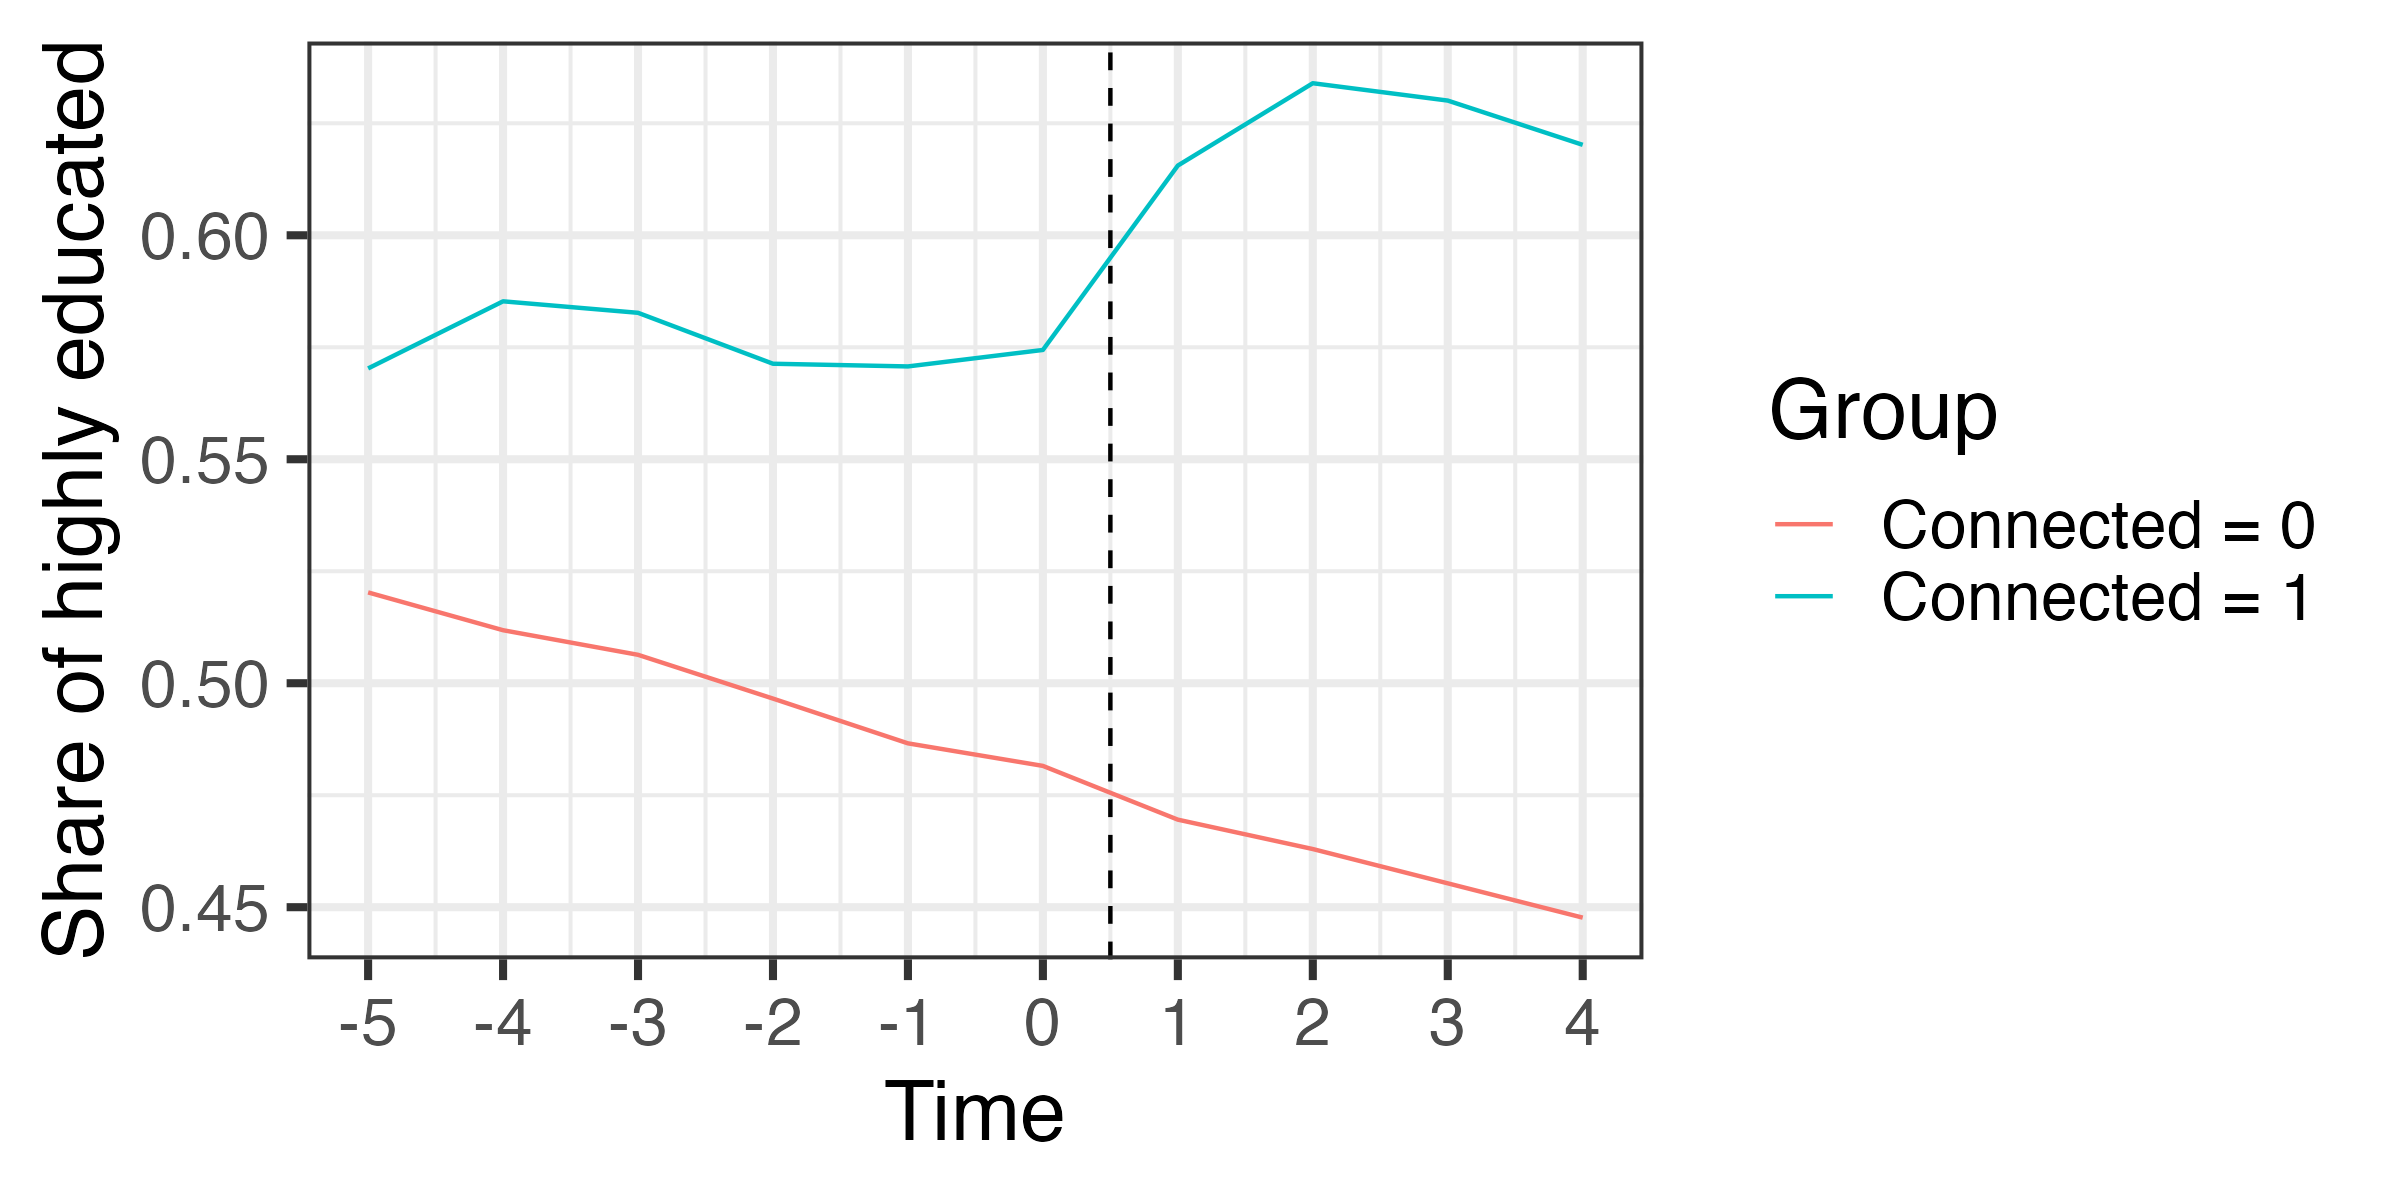
\includegraphics[width=0.75\linewidth]{output/figures/2_common_trends.png}
    \caption{Common trends for education}
    \label{fig:commontrends}
\end{figure}

% Provide a possible explanation for the trends you observe.

\subsection*{(b) Event study}

\begin{figure}[h!]
    \centering
    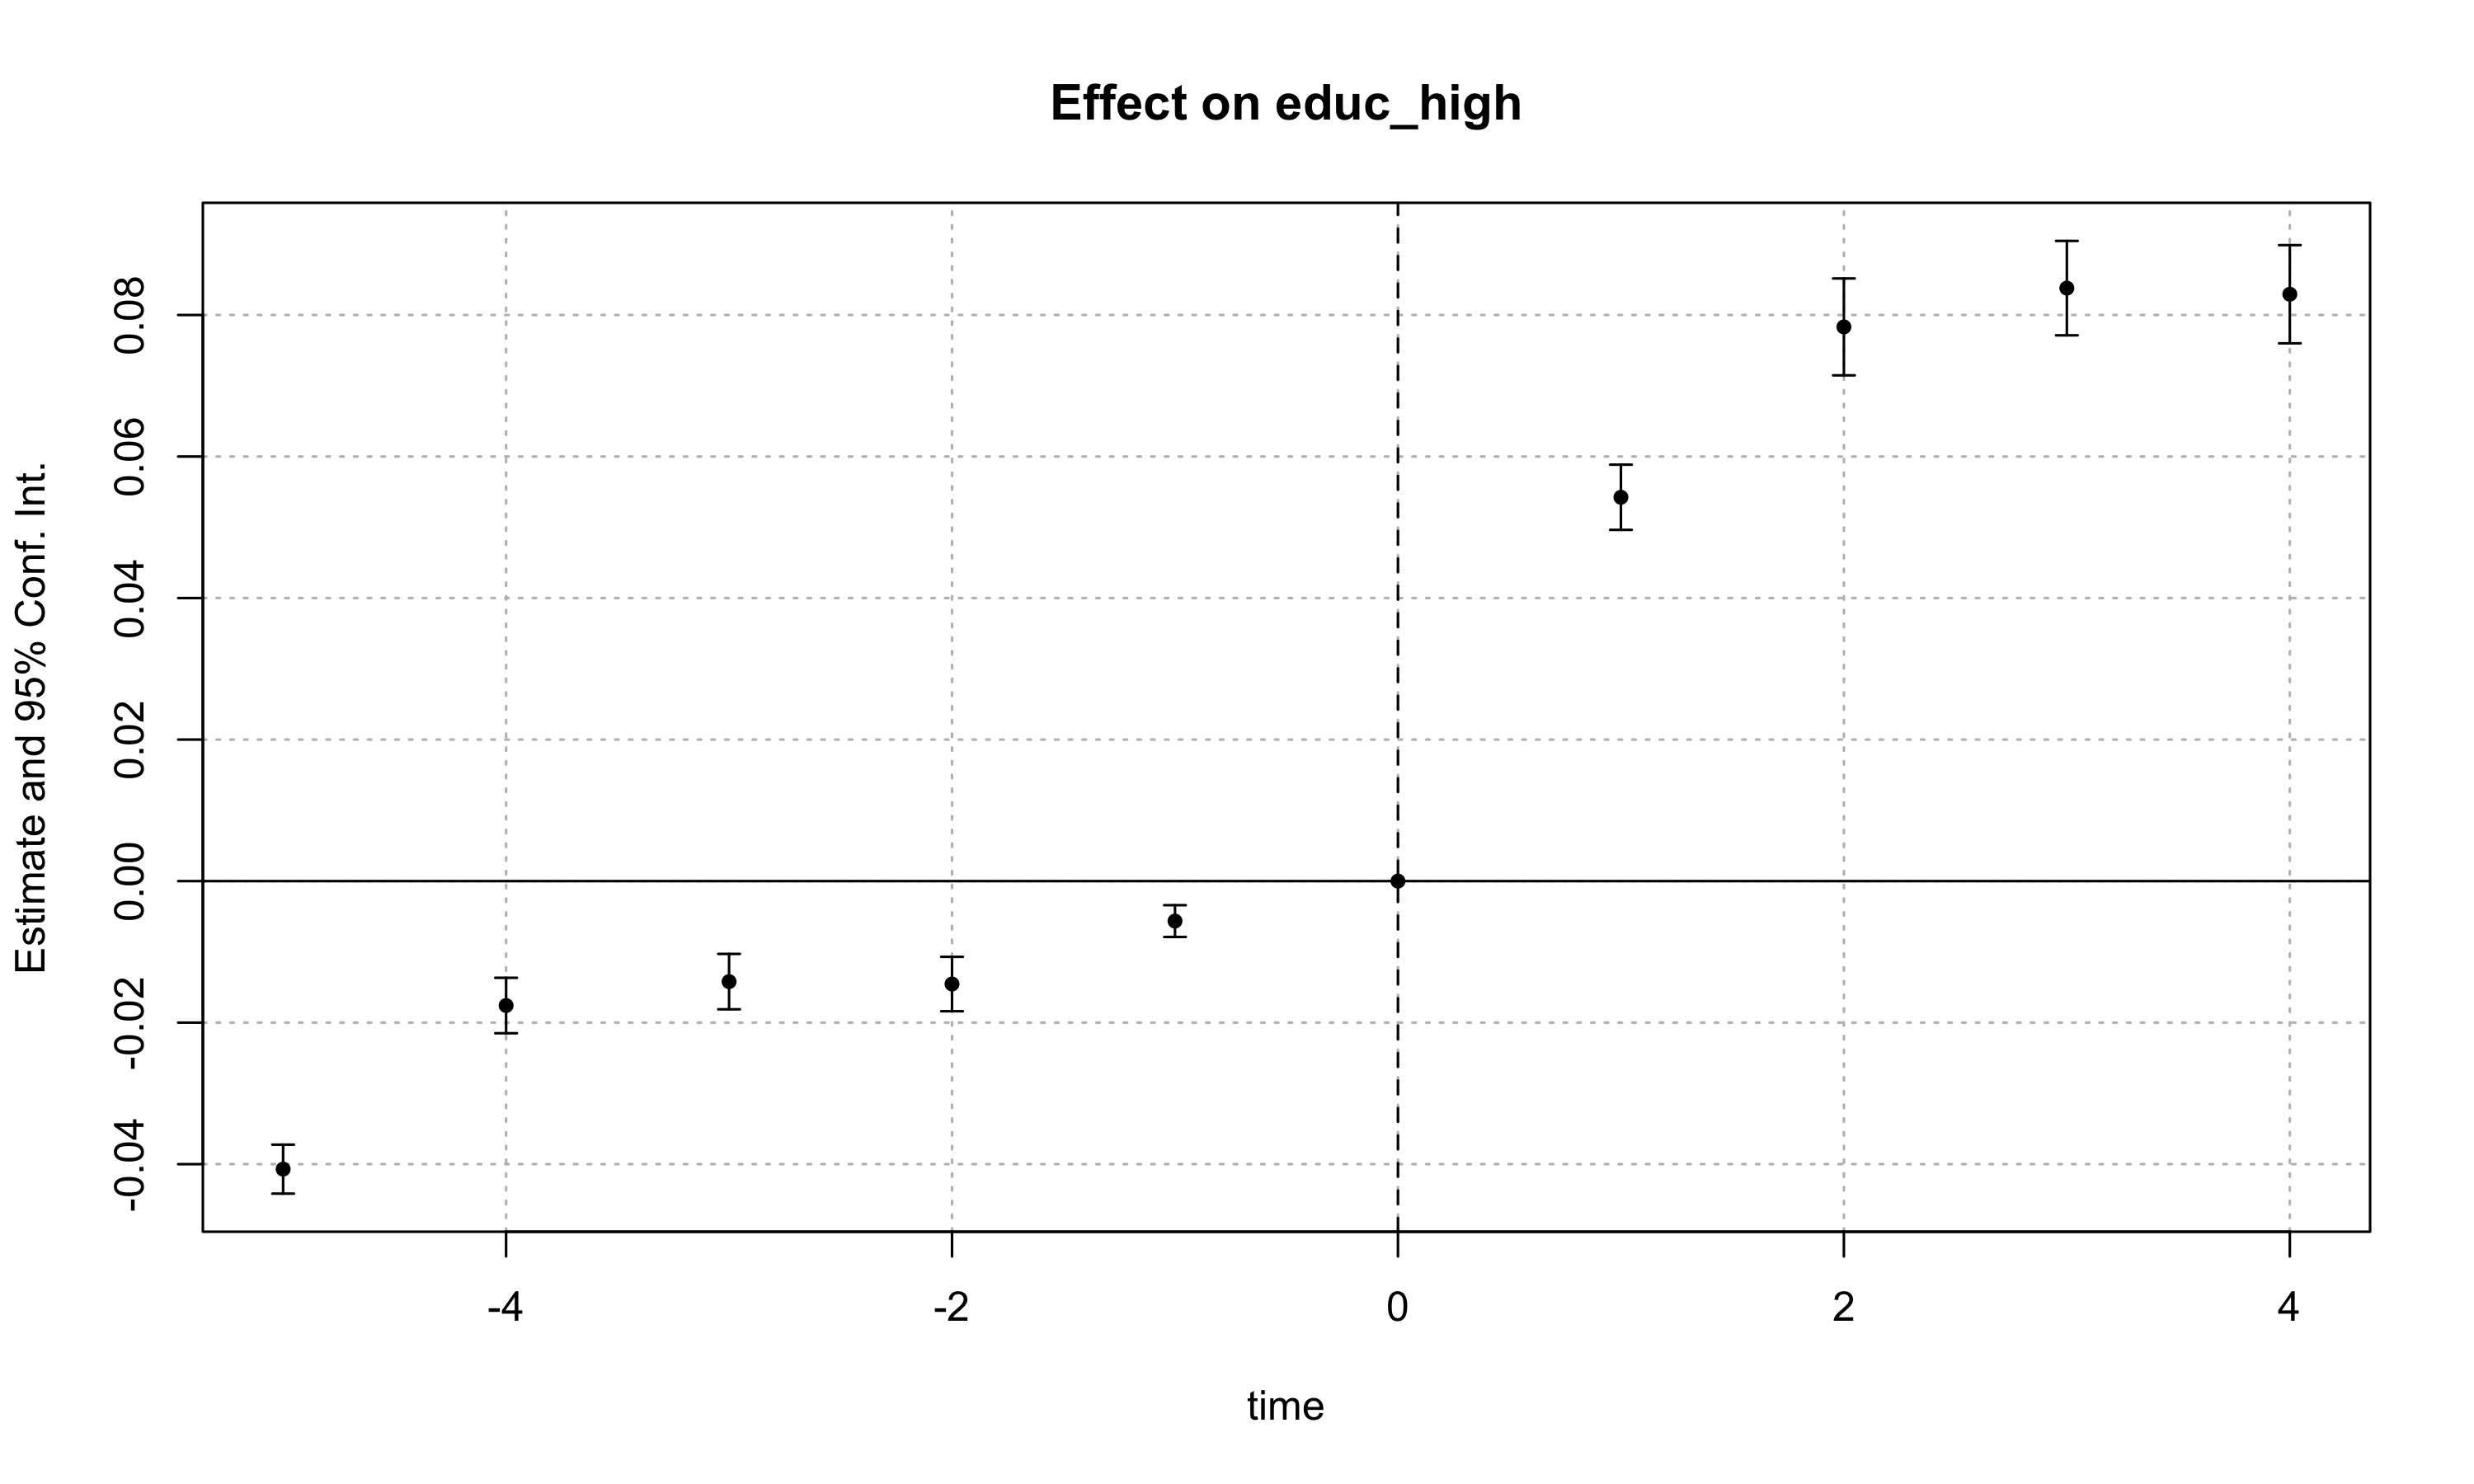
\includegraphics[width=0.75\linewidth]{output/figures/2_event_study.png}
    \caption{Event study: education}
    \label{fig:eventstudy}
\end{figure}

% Conduct an event study for the outcome educ high and report the results in a plot. Based on the results from this and the last question, is it reasonable to use a DiD strategy for this outcome variable?

\subsection*{(c) Bias direction in DiD estimate for education}

% Given the common trend plot above, if you were to estimate the effect of fast internet using a DiD strategy, can we say whether our estimate would be up-ward or downward biased? 

\section*{Question 4}

\subsection*{(a) Clustered bootstrap SE for non-parametric ATET}

\begin{table}[!h]
\centering
\caption{\label{tab:tab:np_atet_clustered}Internet access and employment: Non-parametric bootstrap estimates of ATET, Cluster-robust SEs}
\centering
\begin{tabular}[t]{rrrr}
\toprule
atet & sd & lower\_bound & upper\_bound\\
\midrule
0.0082699 & 0.0093528 & -0.0100616 & 0.0266013\\
\bottomrule
\end{tabular}
\end{table}


% Is the result similar to that in point 1.c?

\section*{Question 5}

\subsection*{(a) Endogeneity concern in regressing labor supply on children}

% Why can’t we just regress female labour supply on the number of children to estimate a causal effect?

\subsection*{(b) IV estimate and treatment interpretation}

% The IV strategy of the authors only identifies a very specific average treatment effect. What is that? Be precise and context-specific

\subsection*{(c) Why OLS over-estimate the negativ effect?}

% Consider columns 1 and 2 in Table 7, which presents OLS and IV estimates, respectively. Provide an explanation for why the OLS estimate are lower than the IV ones (i.e. OLS over-estimates the negative effect).

\end{document}
